%%% Preamble starts here.
\documentclass{amsart}
\usepackage{amsmath}
%for the heading
\usepackage{fancyhdr, enumerate}
%for the picture. 
\usepackage{tikz}
%adjust the page width
\usepackage[margin=1in]{geometry}

\linespread{1.1}

%command for double parentheses
\newcommand{\textmultiset}[2]{\bigl(\!{\binom{#1}{#2}}\!\bigr)}
\newcommand{\displaymultiset}[2]{\left(\!{\binom{#1}{#2}}\!\right)}
\newcommand\multiset[2]{\mathchoice{\displaymultiset{#1}{#2}}
                                {\textmultiset{#1}{#2}}
                                {\textmultiset{#1}{#2}}
                                {\textmultiset{#1}{#2}}}

%special commands for number sets
\def\RR{{\mathbb R}}
\def\NN{{\mathbb N}}
\def\ZZ{{\mathbb Z}}
\def\QQ{{\mathbb Q}}
\def\CC{{\mathbb C}}

% header
\lhead{\sc  Combinatorics: Homework 6}
\chead{\sc Stefano Fochesatto } 
\rhead{\today}
\cfoot{}
\pagestyle{fancy}

%%%% Main document starts here.

\begin{document}
\thispagestyle{fancy}

Reminder: Any time you are asked to answer a question, you need to provide a rigorous justification of your answer. (ie Don't just give a bald answer!)

\begin{enumerate}
%%%first problem
\item (Problem 3.1.7) Let $D_n$ be the number of derangement for a general $n.$ 
	\begin{enumerate}
	\item Calculate $\displaystyle{\lim_{n\to \infty} \frac{D_n}{n!}}$. Interpret your result.\\\\
\noindent\textbf{Answer:} Consider that $D_n$ counts the number of permutations of $[n]$ such that there are no fixed elements. Therefore using inclusion-exclusion principle, we can find a function for $D_n$,
	\begin{equation*}
	D_n = \sum_{k = 0 }^{n} (-1)^{k}(n-k)!{n \choose k}
	\end{equation*}
	From here we can substitute, into the given limit,
	\begin{equation*}
	\displaystyle{\lim_{n\to \infty} \frac{1}{n!}*\sum_{k = 0 }^{n} (-1)^{k}(n-k)!{n \choose k}}
	\end{equation*}
	From here we can simplify the sum for $D_n$,
        \begin{align*}
	\displaystyle{\lim_{n\to \infty} \frac{1}{n!}*\sum_{k = 0 }^{n} (-1)^{k}(n-k)!{n \choose k}} &= 	\displaystyle{\lim_{n\to \infty} \frac{1}{n!}*\sum_{k = 0 }^{n} (-1)^{k}(n-k)!\frac{n!}{k!*(n-k)!}}\\
	&= 
	\displaystyle{\lim_{n\to \infty} \frac{1}{n!}*\sum_{k = 0 }^{n} (-1)^{k}\frac{n!}{k!}}\\
	&=
		\displaystyle{\lim_{n\to \infty} \frac{1}{n!}*(n!)\sum_{k = 0 }^{n} \frac{(-1)^{k}}{k!}}\\
	&=
			\displaystyle{\lim_{n\to \infty} \sum_{k = 0 }^{n} \frac{(-1)^{k}}{k!}}\\
	& = \sum_{k = 0 }^{\infty} \frac{(-1)^{k}}{k!}
	\end{align*}
	Here we need to recognize that the sum that we have is in the form of the power series expansion for $e^x$.
	\begin{equation*}
	e^x = \sum_{k = 0 }^{\infty} \frac{(x)^{k}}{k!}
	\end{equation*}
	We can see that since $x = -1$ we get,
	\begin{equation*}
	\displaystyle{\lim_{n\to \infty} \frac{D_n}{n!}} = \frac{1}{e}
	\end{equation*}
	What we have shown is that $\frac{D_n}{n!}}$ is equivalent to the $n^{th}$ degree Taylor Polynomial of $\frac{1}{e}$. Combinatorially we have show that the ratio of derangements to total permutations converges to $\frac{1}{e}$. 

	
	

\vspace{1in}
	\item Prove that for any $n$, $D_n$ equal the closest integer to $n!/e.$\\
	\noindent\textbf{Answer:} Let's recall the Alternating Series Remainder Theorem, which states that if an alternating series converges to $S$, then the $n^{th}$ partial sum $S_n$ and the corresponding remainder $R_n$ can be defined as follows,
	\begin{equation*}
	S_n+R_n = S
	\end{equation*}
	Such that,
	\begin{align*}
	S_n &=  \sum_{k = 1 }^{n} (-1)^{k+1}a_k \\
	R_n &=  \sum_{k = n+1 }^{\infity} (-1)^{k+1}a_k 
	\end{align*}
	Then by substitution we know that,
	\begin{equation*}
	R_n = S - \sum_{k = 1 }^{n} (-1)^{k+1}a_k 
	\end{equation*}
	What we are being asked to prove is,
	\begin{equation*}
	\lvert{\frac{n!}{e}-D_n\rvert < \frac{1}{2}
	\end{equation*}
	For all $n$. Since we have proven that $D_n$ converges to $\frac{n!}{e}$, it must be true that as $n$ increases the remainder gets smaller and smaller, as one would expect. So let $n = 1$ and, through some algebra we get, 
	\begin{align*}
	\frac{1!}{e} - n! \sum_{k = 0 }^{1} \frac{(-1)^{k}}{k!} &= \frac{1!}{e} - (1!)*(1-1)\\
	 &= \frac{1}{e}
	\end{align*}
	Thus since $\frac{1}{e} < \frac{1}{2}$  the statement holds for all $n \geq 1$.



	
	
	\\
	\vspace{1in}
	\end{enumerate}

\item (Problem 3.1.9) Generalize the previous problem: In how many ways can you distribute $k$ identical objects to $n$ distinct recipients so that each recipient receives at most $r$ objects?\\
\noindent\textbf{Answer:}  Let $P_i$ be the property that $i^{th}$ recipient receives $r+1$ or more objects. Therefore we want a formula for $N_{=}(\theta)$. Using Inclusion-Exclusion we get 
\begin{equation*}
N_{=}(\theta) = \sum_{i = 0}^{n} (-1)^{i} {n\choose i}{\multiset{n}{k - i(r+1)}} 
\end{equation*}



  \\
	\vspace{1in}

\item (Problem 3.1.17)  A taxi drives from the intersection labeled $A$ to the intersection labeled $B$ in the grid of streets shown below. The driver only drives north (up) ie east (right).

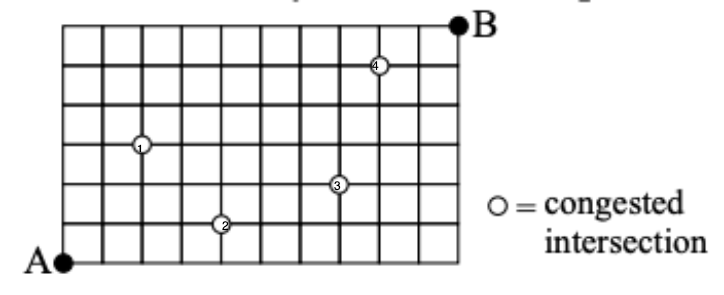
\includegraphics[scale=0.4]{pic.png}

Traffic reports indicate that there is heavy congestion at the intersections identified. How many routes from $A$ to $B$ can the driver take that ...\\
	\begin{enumerate}
	\item avoid all congested intersections?\\
	\noindent\textbf{Answer:} }  Let $P_i$ be the property that a route has the $i^{th}$ congested intersection. Therefore we want a formula for $N_{=}(\theta)$. 
	\begin{align*}
	N_{=}(\theta) &= p_0 - ((p_{1}+p_{2}+p_{3}+p_{4}) - (p_{14}+p_{23}+p_{24}+p_{34}) - 2(p_{123}))\\ 	
	& = 8008-9081+3022+480\\
	& = 2429
	\end{align*}
%% {5 \choose 3}{11\choose 3} - {5 \choose 1}{11 \choose 5} - {9 \choose 2}{7 \choose 4} - {13\choose 5}{3 \choose 1}
	
	%%- 2459+3022 + 480
	
	
	\vspace{1in}
	\item pass through at most one congested intersection?\\
	\noindent\textbf{Answer:} Consider inclusion exclusion such that we want $N_{\leq}(1)$. Therefore
	\begin{align*}
	N_{\leq}(1) &= p_0 - ((p_{14}+p_{23}+p_{24}+p_{34}) - (2p_{123}))\\
	 & = 8008 - 3022 + 480\\
	 & = 5466
	\end{align*}
	\vspace{1in}
	\end{enumerate}

\end{enumerate}
\end{document}
